\documentclass{article}
\usepackage{graphicx} % new way of doing eps files
\usepackage{listings} % nice code layout
\usepackage[usenames]{color} % color
\definecolor{listinggray}{gray}{0.9}
\definecolor{graphgray}{gray}{0.7}
\definecolor{ans}{rgb}{1,0,0}
\definecolor{blue}{rgb}{0,0,1}
% \Verilog{title}{label}{file}
\newcommand{\Verilog}[3]{
  \lstset{language=Verilog}
  \lstset{backgroundcolor=\color{listinggray},rulecolor=\color{blue}}
  \lstset{linewidth=\textwidth}
  \lstset{commentstyle=\textit, stringstyle=\upshape,showspaces=false}
  \lstset{frame=tb}
  \lstinputlisting[caption={#1},label={#2}]{#3}
}


\author{your names}
\title{Lab title}

\begin{document}
\maketitle

\section{Executive Summary}
The Executive Summary section should be a single concise paragraph that describes:
\begin{enumerate}
	\item The goal of the lab
	\item What modules you created and what they do.  This should describe how the modules function and how they fit into the overall processor that we are building.  For instance, for Lab 1, you will want to describe the operation of the register and the fact that it is used to store the program counter, which is used to keep track of which instruction to execute next.
	\item Whether your lab was successful.  If not successful, please state what is not currently working.
\end{enumerate}	

\section{Test Report}
To verify operation of this/these module(s), this lab requires N number of test benches.
\begin{enumerate}
	\item Register Test Bench
\end{enumerate}

\subsection{Register Test Bench}
The register test bench contains:
\begin{enumerate}
	\item Inputs
	\begin{enumerate}
		\item name\_of\_input - phrase describing the input
		\item name\_of\_input - phrase describing the input
	\end{enumerate}	
	\item Outputs
	\begin{enumerate}	
		\item name\_of\_output - phrase describing the output
	\end{enumerate}
\end{enumerate} 

Briefly describe what the testbench does and what it is testing.  In something as simple as Lab 1, this might be as short as a few sentences sentences.   

Operation of the testbench is verified by comparing the Simulation Results with the Expected Results Table (you can just include this sentence).  Next you should state whether the module works as expected.  If not, please describe what does not work and why it does not work.

\begin{figure}
	\begin{center}
		\caption{Expected Results of the register test.}\label{fig:ert_registertest}
		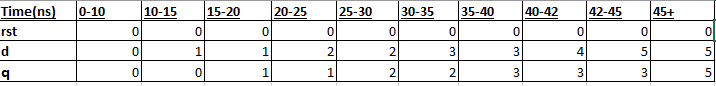
\includegraphics[width=1.0\textwidth]{../images/ert_register_test.png}
	\end{center}
\end{figure}

\begin{figure}
	\begin{center}
		\caption{Timing diagram for the register test.}\label{fig:registertest}
		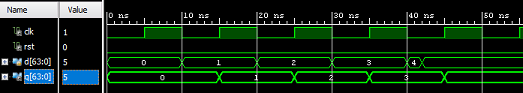
\includegraphics[width=1.0\textwidth]{../images/register_test.png}
	\end{center}
\end{figure}


\pagebreak

\section{Code Appendix}
\Verilog{Verilog code for implementing a register.}{code:reg}{../code/1_fetch/register.v}
\Verilog{Verilog code for testing a register.}{code:regtest}{../code/1_fetch/register_test.v}
\end{document} 